\documentclass[tikz,border=10pt]{standalone}
\usepackage{fontspec}
\setmainfont{Arial}[SmallCapsFont={Latin Modern Roman}]
\setsansfont{Arial}
\usepackage{amsmath, amssymb, bm}
\usepackage{tikz}
\usetikzlibrary{arrows.meta}

% ============================================================
% Custom colors
% ============================================================
\definecolor{boxBorder}{HTML}{5B676F}
\definecolor{colHeader}{HTML}{393950}
\definecolor{textMain}{HTML}{2C2C2C}
\definecolor{textSub}{HTML}{5B676F}
\definecolor{enhanced}{HTML}{DF8A2C}
\definecolor{newStar}{HTML}{2C2C2C}
\definecolor{mvPurple}{HTML}{7A6AAD}
\definecolor{susieBlue}{HTML}{4990E1}
\definecolor{ashRed}{HTML}{E53934}
\definecolor{infGreen}{HTML}{7BB342}

\begin{document}

% ============================================================
% Panel A: susieR 2.0 Software Architecture
% Gray neutral base, Refinement+Output column gets warm accent
% ============================================================
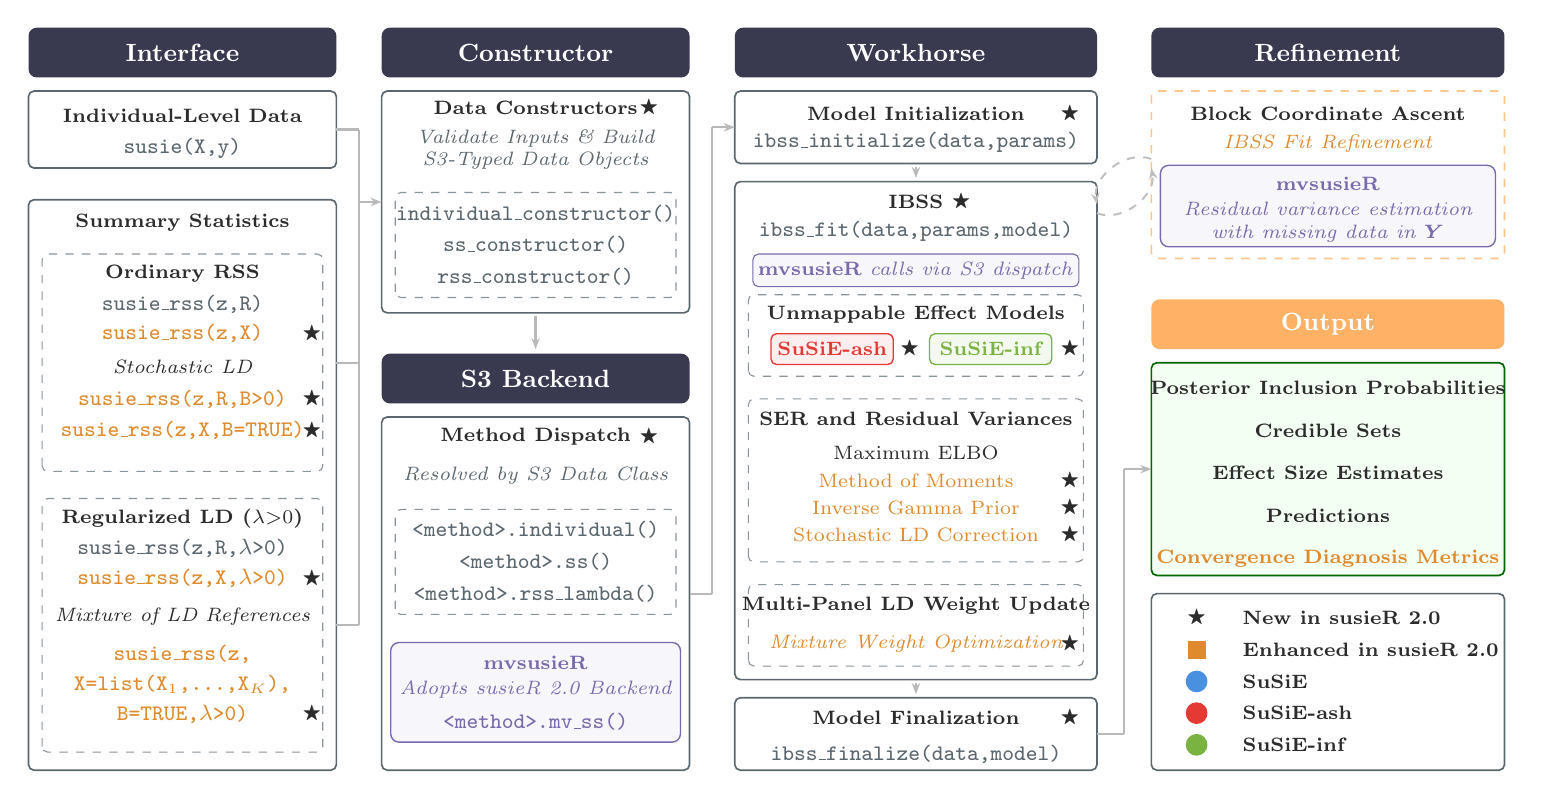
\begin{tikzpicture}[
    x=1.15cm, y=1.15cm,
    >={Stealth[length=4pt, width=3pt]},
    font=\sffamily,
    %% --- Reusable styles ---
    % Box styles
    solidbox/.style={boxBorder, rounded corners=2pt, line width=0.6pt, fill=white},
    dashbox/.style={boxBorder, rounded corners=2pt, line width=0.4pt, dashed, opacity=0.7},
    % Arrow styles
    arrowline/.style={draw=gray!55, line width=0.8pt, ->},
    busline/.style={draw=gray!55, line width=0.8pt},
    dashedarrow/.style={draw=gray!50, line width=0.7pt, dashed, ->},
    % Text styles
    colheader/.style={font=\bfseries\small, text=white},
    boxtitle/.style={font=\bfseries\scriptsize, text=textMain},
    codestyle/.style={font=\ttfamily\fontsize{7.75}{9.3}\selectfont, text=textSub},
    subtitle/.style={font=\itshape\scriptsize, text=textSub},
    enhtext/.style={font=\scriptsize, text=enhanced},
    enhcode/.style={font=\ttfamily\fontsize{7.75}{9.3}\selectfont, text=enhanced},
    enhbold/.style={font=\bfseries\scriptsize, text=enhanced},
    starmark/.style={font=\scriptsize, text=newStar},
    mvlabel/.style={font=\bfseries\scriptsize, text=mvPurple},
    mvtext/.style={font=\itshape\scriptsize, text=mvPurple},
    mvcode/.style={font=\ttfamily\fontsize{7.75}{9.3}\selectfont, text=mvPurple},
]

% ============================================================
% COLUMN HEADERS  (uniform dark gray)
% ============================================================
\fill[colHeader, rounded corners=3pt] (0.35,8.55) rectangle (3.75,9.10);
\node[colheader] at (2.05,8.825) {Interface};

\fill[colHeader, rounded corners=3pt] (4.25,8.55) rectangle (7.65,9.10);
\node[colheader] at (5.95,8.825) {Constructor};

\fill[colHeader, rounded corners=3pt] (8.15,8.55) rectangle (12.15,9.10);
\node[colheader] at (10.15,8.825) {Workhorse};

\fill[colHeader, rounded corners=3pt] (12.75,8.55) rectangle (16.65,9.10);
\node[colheader] at (14.70,8.825) {Refinement};

% ============================================================
% 1. INTERFACE COLUMN
% ============================================================

% --- Individual-Level Data ---
\draw[solidbox] (0.35,7.55) rectangle (3.75,8.40);
\node[boxtitle] at (2.05,8.13) {Individual-Level Data};
\node[codestyle] at (2.05,7.77) {susie(X,y)};

% --- Summary Statistics outer box ---
\draw[solidbox] (0.35,0.90) rectangle (3.75,7.20);
\node[boxtitle] at (2.05,6.95) {Summary Statistics};

\def\sL{0.50}
\def\sR{3.60}
\pgfmathsetmacro{\sCx}{(\sL+\sR)/2}

% -- Ordinary RSS --
\draw[dashbox] (\sL,4.20) rectangle (\sR,6.60);
\node[boxtitle] at (\sCx,6.38) {Ordinary RSS};
\node[codestyle] at (\sCx,6.05) {susie\_rss(z,R)};
\node[enhcode] at (\sCx,5.72) {susie\_rss(z,X)};
\node[starmark] at (3.48,5.72) {$\bigstar$};
\node[font=\itshape\scriptsize, text=textMain] at (\sCx,5.35) {Stochastic LD};
\node[enhcode] at (\sCx,5.00) {susie\_rss(z,R,B{>}0)};
\node[starmark] at (3.48,5.00) {$\bigstar$};
\node[enhcode] at (\sCx,4.65) {susie\_rss(z,X,B=TRUE)};
\node[starmark] at (3.48,4.65) {$\bigstar$};

% -- Regularized LD --
\draw[dashbox] (\sL,1.10) rectangle (\sR,3.90);
\node[boxtitle] at (\sCx,3.68) {Regularized LD ($\lambda{>}0$)};
\node[codestyle] at (\sCx,3.35) {susie\_rss(z,R,$\lambda${>}0)};
\node[enhcode] at (\sCx,3.02) {susie\_rss(z,X,$\lambda${>}0)};
\node[starmark] at (3.48,3.02) {$\bigstar$};
\node[font=\itshape\scriptsize, text=textMain, text width=3.5cm, align=center]
    at (\sCx,2.60) {Mixture of LD References};
\node[enhcode] at (\sCx,2.18) {susie\_rss(z,};
\node[enhcode] at (\sCx,1.85) {X=list(X$_1$,\ldots,X$_K$),};
\node[enhcode] at (\sCx,1.52) {B=TRUE,$\lambda${>}0)};
\node[starmark] at (3.48,1.52) {$\bigstar$};


% ============================================================
% 2. CONSTRUCTOR COLUMN
% ============================================================

% --- Data Constructors ---
\draw[solidbox] (4.25,5.95) rectangle (7.65,8.40);
\node[boxtitle] at (5.95,8.22) {Data Constructors};
\node[starmark] at (7.20,8.22) {$\bigstar$};
\node[subtitle, text width=3.5cm, align=center]
    at (5.95,7.75) {Validate Inputs \& Build \\S3-Typed Data Objects};
\draw[dashbox] (4.40,6.12) rectangle (7.50,7.28);
\node[codestyle] at (5.95,7.05) {individual\_constructor()};
\node[codestyle] at (5.95,6.70) {ss\_constructor()};
\node[codestyle] at (5.95,6.35) {rss\_constructor()};

% --- Arrow ---
\draw[arrowline] (5.95,5.92) -- (5.95,5.55);

% --- S3 Backend bar ---
\fill[colHeader, rounded corners=3pt] (4.25,4.95) rectangle (7.65,5.50);
\node[colheader] at (5.95,5.225) {S3 Backend};

% --- Method Dispatch ---
\draw[solidbox] (4.25,0.90) rectangle (7.65,4.80);
\node[boxtitle] at (5.95,4.58) {Method Dispatch};
\node[starmark] at (7.20,4.58) {$\bigstar$};
\node[subtitle] at (5.95,4.15) {Resolved by S3 Data Class};
\draw[dashbox] (4.40,2.62) rectangle (7.50,3.78);
\node[codestyle] at (5.95,3.55) {<method>.individual()};
\node[codestyle] at (5.95,3.20) {<method>.ss()};
\node[codestyle] at (5.95,2.85) {<method>.rss\_lambda()};

% --- mvsusieR pill ---
\draw[mvPurple, rounded corners=3pt, line width=0.5pt, fill=mvPurple!6]
    (4.35,1.21) rectangle (7.55,2.31);
\node[mvlabel] at (5.95,2.09) {mvsusieR};
\node[mvtext] at (5.95,1.79) {Adopts susieR 2.0 Backend};
\node[mvcode] at (5.95,1.43) {<method>.mv\_ss()};


% ============================================================
% 3. WORKHORSE COLUMN
% ============================================================

% --- Model Initialization ---
\draw[solidbox] (8.15,7.60) rectangle (12.15,8.40);
\node[boxtitle] at (10.15,8.15) {Model Initialization};
\node[starmark] at (11.85,8.15) {$\bigstar$};
\node[codestyle] at (10.15,7.83) {ibss\_initialize(data,params)};

% --- Arrow ---
\draw[arrowline] (10.15,7.56) -- (10.15,7.44);

% --- IBSS large box ---
\draw[solidbox] (8.15,1.90) rectangle (12.15,7.40);
\node[boxtitle] at (10.15,7.18) {IBSS};
\node[starmark] at (10.65,7.18) {$\bigstar$};
\node[codestyle] at (10.15,6.85) {ibss\_fit(data,params,model)};

% mvsusieR shared note
\draw[mvPurple, rounded corners=2pt, line width=0.4pt, fill=mvPurple!6]
    (8.35,6.24) rectangle (11.95,6.60);
\node[font=\scriptsize, text=mvPurple]
    at (10.15,6.42) {\textbf{mvsusieR} \textit{calls via S3 dispatch}};

\def\wL{8.30}
\def\wR{12.00}
\pgfmathsetmacro{\wCx}{(\wL+\wR)/2}

% -- Unmappable Effect Models --
\draw[dashbox] (\wL,5.25) rectangle (\wR,6.15);
\node[boxtitle] at (\wCx,5.93) {Unmappable Effect Models};

% SuSiE-ash pill
\draw[ashRed, rounded corners=2pt, line width=0.5pt, fill=ashRed!8]
    (8.55,5.38) rectangle (9.90,5.72);
\node[font=\bfseries\scriptsize, text=ashRed] at (9.225,5.55) {SuSiE-ash};
\node[starmark] at (10.08,5.55) {$\bigstar$};

% SuSiE-inf pill
\draw[infGreen, rounded corners=2pt, line width=0.5pt, fill=infGreen!8]
    (10.30,5.38) rectangle (11.65,5.72);
\node[font=\bfseries\scriptsize, text=infGreen] at (10.975,5.55) {SuSiE-inf};
\node[starmark] at (11.85,5.55) {$\bigstar$};

% -- Residual Variance Estimation --
\draw[dashbox] (\wL,3.20) rectangle (\wR,5.00);
\node[boxtitle] at (\wCx,4.78) {SER and Residual Variances};
\node[font=\scriptsize, text=textMain] at (\wCx,4.40) {Maximum ELBO};
\node[enhtext] at (\wCx,4.10) {Method of Moments};
\node[starmark] at (11.85,4.10) {$\bigstar$};
\node[enhtext] at (\wCx,3.80) {Inverse Gamma Prior};
\node[starmark] at (11.85,3.80) {$\bigstar$};
\node[enhtext] at (\wCx,3.50) {Stochastic LD Correction};
\node[starmark] at (11.85,3.50) {$\bigstar$};

% -- Multi-Panel LD Weight Update --
\draw[dashbox] (\wL,2.05) rectangle (\wR,2.95);
\node[boxtitle] at (\wCx,2.72) {Multi-Panel LD Weight Update};
\node[font=\itshape\scriptsize, text=enhanced] at (\wCx,2.30) {Mixture Weight Optimization};
\node[starmark] at (11.85,2.30) {$\bigstar$};

% --- Arrow ---
\draw[arrowline] (10.15,1.86) -- (10.15,1.74);

% --- Model Finalization ---
\draw[solidbox] (8.15,0.90) rectangle (12.15,1.70);
\node[boxtitle] at (10.15,1.48) {Model Finalization};
\node[starmark] at (11.85,1.48) {$\bigstar$};
\node[codestyle] at (10.15,1.08) {ibss\_finalize(data,model)};


% ============================================================
% 4. REFINEMENT + OUTPUT COLUMN  (warm accent)
% ============================================================

% --- Block Coordinate Ascent ---
\draw[orange!45, rounded corners=2pt, line width=0.6pt, dashed]
    (12.75,6.55) rectangle (16.65,8.40);
\node[boxtitle] at (14.70,8.15) {Block Coordinate Ascent};
\node[font=\itshape\scriptsize, text=enhanced] at (14.70,7.82) {IBSS Fit Refinement};

% mvsusieR pill inside BCA
\draw[mvPurple, rounded corners=3pt, line width=0.5pt, fill=mvPurple!6]
    (12.85,6.68) rectangle (16.55,7.58);
\node[mvlabel] at (14.70,7.38) {mvsusieR};
\node[mvtext] at (14.70,7.10) {Residual variance estimation};
\node[mvtext] at (14.70,6.82) {with missing data in $\bm{Y}$};

% --- Output header (warm) ---
\fill[orange!60, rounded corners=3pt] (12.75,5.55) rectangle (16.65,6.10);
\node[colheader] at (14.70,5.825) {Output};

% --- Output content box ---
\draw[green!40!black, rounded corners=2pt, line width=0.6pt, fill=green!5]
    (12.75,3.05) rectangle (16.65,5.40);
\node[font=\bfseries\scriptsize, text=textMain] at (14.70,5.12) {Posterior Inclusion Probabilities};
\node[font=\bfseries\scriptsize, text=textMain] at (14.70,4.65) {Credible Sets};
\node[font=\bfseries\scriptsize, text=textMain] at (14.70,4.18) {Effect Size Estimates};
\node[font=\bfseries\scriptsize, text=textMain] at (14.70,3.71) {Predictions};
\node[enhbold] at (14.70,3.24) {Convergence Diagnosis Metrics};

% --- Legend box ---
\draw[solidbox] (12.75,0.90) rectangle (16.65,2.85);

\def\lMx{13.25}
\def\lTx{13.65}

\node[starmark] at (\lMx,2.58) {$\bigstar$};
\node[font=\bfseries\scriptsize, text=textMain, anchor=west] at (\lTx,2.58) {New in susieR 2.0};

\fill[enhanced] (\lMx-0.10,2.23-0.10) rectangle (\lMx+0.10,2.23+0.10);
\node[font=\bfseries\scriptsize, text=textMain, anchor=west] at (\lTx,2.23) {Enhanced in susieR 2.0};

\fill[susieBlue] (\lMx,1.88) circle (0.12);
\node[font=\bfseries\scriptsize, text=textMain, anchor=west] at (\lTx,1.88) {SuSiE};

\fill[ashRed] (\lMx,1.53) circle (0.12);
\node[font=\bfseries\scriptsize, text=textMain, anchor=west] at (\lTx,1.53) {SuSiE-ash};

\fill[infGreen] (\lMx,1.18) circle (0.12);
\node[font=\bfseries\scriptsize, text=textMain, anchor=west] at (\lTx,1.18) {SuSiE-inf};


% ============================================================
% 5. ARROWS
% ============================================================

% --- Interface -> Constructor bus ---
\pgfmathsetmacro{\busX}{4.00}
\pgfmathsetmacro{\iMid}{(7.55+8.40)/2}
\pgfmathsetmacro{\sMidA}{(4.20+6.60)/2}
\pgfmathsetmacro{\sMidB}{(1.10+3.90)/2}

\draw[busline] (3.75,\iMid) -- (\busX,\iMid);
\draw[busline] (3.75,\sMidA) -- (\busX,\sMidA);
\draw[busline] (3.75,\sMidB) -- (\busX,\sMidB);
\draw[busline] (\busX,\iMid) -- (\busX,\sMidB);
\pgfmathsetmacro{\dcMid}{(5.95+8.40)/2}
\draw[arrowline] (\busX,\dcMid) -- (4.25,\dcMid);

% --- Constructor -> Workhorse ---
\pgfmathsetmacro{\mdMid}{(0.90+4.80)/2}
\pgfmathsetmacro{\wiMid}{(7.60+8.40)/2}
\pgfmathsetmacro{\elbX}{7.90}
\draw[busline] (7.65,\mdMid) -- (\elbX,\mdMid);
\draw[busline] (\elbX,\mdMid) -- (\elbX,\wiMid);
\draw[arrowline] (\elbX,\wiMid) -- (8.15,\wiMid);

% --- IBSS <-> BCA iteration loop ---
\draw[dashedarrow] (12.15,7.05) to[bend right=60] (12.75,7.55);
\draw[dashedarrow] (12.75,7.65) to[bend right=60] (12.15,7.15);

% --- Model Finalization -> Output ---
\pgfmathsetmacro{\finMid}{(0.90+1.70)/2}
\pgfmathsetmacro{\outMid}{(3.05+5.40)/2}
\pgfmathsetmacro{\foElb}{12.45}
\draw[busline] (12.15,\finMid) -- (\foElb,\finMid);
\draw[busline] (\foElb,\finMid) -- (\foElb,\outMid);
\draw[arrowline] (\foElb,\outMid) -- (12.75,\outMid);

\end{tikzpicture}

\end{document}
